\documentclass[border=8pt,tikz]{standalone}
\usepackage{amsmath,amssymb}
\usepackage{tikz}
\usetikzlibrary{arrows.meta,calc,decorations.pathreplacing,patterns,shapes.geometric,positioning,shadings,plotmarks}

\begin{document}
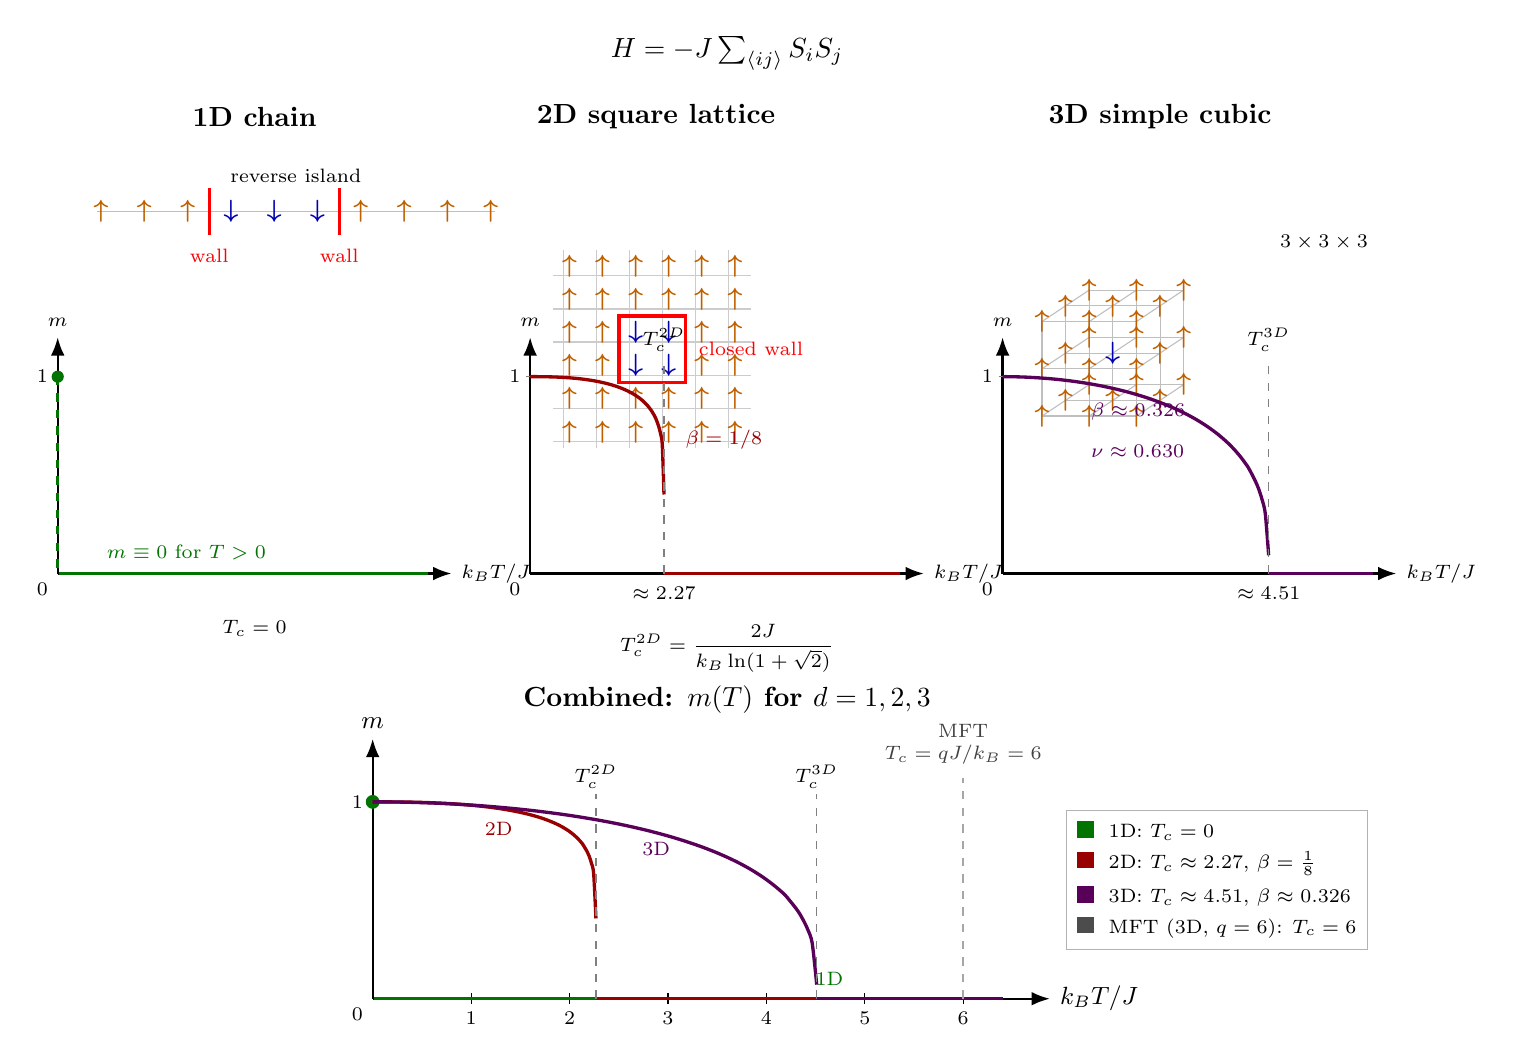
\begin{tikzpicture}[>=Latex,font=\small]

% =====================================================
% Spin arrow macros
% Up = +1 (dark orange), Down = -1 (dark blue)
% =====================================================
\def\upS{\textcolor{orange!75!black}{$\boldsymbol{\uparrow}$}}
\def\dnS{\textcolor{blue!70!black}{$\boldsymbol{\downarrow}$}}

% Top header: Hamiltonian
\node[font=\normalsize] at (8.5, 6.6) {$H = -J \sum_{\langle ij\rangle} S_i S_j$};

% =====================================================
% LEFT PANEL: 1D chain
% =====================================================
\begin{scope}[xshift=0cm,yshift=0cm]
  \node[font=\bfseries] at (2.5, 5.8) {1D chain};

  \def\dx{0.55}
  \draw[gray!50,thin] (0.9*\dx, 4.6) -- (10.1*\dx, 4.6);
  \foreach \i in {1,2,3,7,8,9,10} {
    \node at (\i*\dx, 4.6) {\upS};
  }
  \foreach \i in {4,5,6} {
    \node at (\i*\dx, 4.6) {\dnS};
  }
  % domain wall markers (between 3-4 and 6-7)
  \draw[red,very thick] (3.5*\dx, 4.30) -- (3.5*\dx, 4.90);
  \draw[red,very thick] (6.5*\dx, 4.30) -- (6.5*\dx, 4.90);
  \node[red,font=\scriptsize,anchor=north] at (3.5*\dx, 4.25) {wall};
  \node[red,font=\scriptsize,anchor=north] at (6.5*\dx, 4.25) {wall};
  \node[font=\scriptsize] at (5.5*\dx, 5.05) {reverse island};

  % m(T) plot for 1D
  \draw[->,thick] (0,0) -- (5.0,0) node[right,font=\scriptsize] {$k_B T/J$};
  \draw[->,thick] (0,0) -- (0,3.0) node[above,font=\scriptsize] {$m$};
  \node[font=\scriptsize,anchor=north east] at (0,0) {$0$};
  \node[font=\scriptsize,anchor=east] at (0,2.5) {$1$};
  \draw[thin,gray] (-0.05,2.5) -- (0.05,2.5);
  \draw[very thick,green!45!black] (0.02,0) -- (4.7,0);
  \fill[green!45!black] (0,2.5) circle (2.2pt);
  \draw[very thick,green!45!black,dashed] (0,2.5) -- (0,0);
  \node[font=\scriptsize,green!45!black,anchor=south west] at (0.5,0.05) {$m\equiv 0$ for $T>0$};
  \node[font=\scriptsize] at (2.5,-0.7) {$T_c = 0$};
\end{scope}

% =====================================================
% MIDDLE PANEL: 2D 6x6 lattice
% =====================================================
\begin{scope}[xshift=6.0cm,yshift=0cm]
  \node[font=\bfseries] at (1.6, 5.8) {2D square lattice};

  \def\cs{0.42}
  % grid background
  \draw[gray!40,thin] (0.5-0.5*\cs,1.8-0.5*\cs) grid[step=\cs] (0.5+5.5*\cs,1.8+5.5*\cs);
  % Spins: rows from r=0 (bottom) to r=5 (top); island at c=2,3 r=2,3
  \foreach \r in {0,1,2,3,4,5} {
    \foreach \c in {0,1,2,3,4,5} {
      \pgfmathtruncatemacro{\isdown}{ ((\c==2 || \c==3) && (\r==2 || \r==3)) ? 1 : 0 }
      \ifnum\isdown=1
        \node at (\c*\cs+0.5, \r*\cs+1.8) {\dnS};
      \else
        \node at (\c*\cs+0.5, \r*\cs+1.8) {\upS};
      \fi
    }
  }
  % closed domain wall around the 2x2 island
  \draw[red,very thick]
    (0.5+1.5*\cs, 1.8+1.5*\cs) rectangle (0.5+3.5*\cs, 1.8+3.5*\cs);
  \node[red,font=\scriptsize,anchor=west] at (0.5+3.5*\cs+0.05, 1.8+2.5*\cs) {closed wall};

  % m(T) plot for 2D
  \draw[->,thick] (0,0) -- (5.0,0) node[right,font=\scriptsize] {$k_B T/J$};
  \draw[->,thick] (0,0) -- (0,3.0) node[above,font=\scriptsize] {$m$};
  \node[font=\scriptsize,anchor=north east] at (0,0) {$0$};
  \node[font=\scriptsize,anchor=east] at (0,2.5) {$1$};
  \draw[thin,gray] (-0.05,2.5) -- (0.05,2.5);
  \def\Tcd{1.70}
  \draw[very thick,red!60!black] plot[smooth,samples=80,domain=0.0:\Tcd]
     (\x, {2.5*((1 - (\x/\Tcd)^2.5)^(0.125))});
  \draw[very thick,red!60!black] (\Tcd,0) -- (4.7,0);
  \draw[gray,dashed,thin] (\Tcd,0) -- (\Tcd,2.7);
  \node[font=\scriptsize,anchor=south] at (\Tcd,2.7) {$T_c^{2D}$};
  \node[font=\scriptsize,anchor=north] at (\Tcd,-0.05) {$\approx 2.27$};
  \node[font=\scriptsize,red!60!black,anchor=west] at (1.85,1.7) {$\beta = 1/8$};
  \node[font=\scriptsize,align=center] at (2.5,-0.95)
    {$T_c^{2D} = \dfrac{2J}{k_B \ln(1+\sqrt{2})}$};
\end{scope}

% =====================================================
% RIGHT PANEL: 3D simple cubic
% =====================================================
\begin{scope}[xshift=12.0cm,yshift=0cm]
  \node[font=\bfseries] at (2.0, 5.8) {3D simple cubic};

  \def\ax{0.6}
  \def\ay{0.6}
  \def\axd{0.30}
  \def\ayd{0.20}
  \def\bx{0.5}
  \def\by{2.0}

  % wires
  \foreach \k in {2,1,0} {
    \foreach \j in {0,1,2} {
      \draw[gray!50,thin]
        ({\bx + 0*\ax + \k*\axd}, {\by + \j*\ay + \k*\ayd})
        -- ({\bx + 2*\ax + \k*\axd}, {\by + \j*\ay + \k*\ayd});
    }
    \foreach \i in {0,1,2} {
      \draw[gray!50,thin]
        ({\bx + \i*\ax + \k*\axd}, {\by + 0*\ay + \k*\ayd})
        -- ({\bx + \i*\ax + \k*\axd}, {\by + 2*\ay + \k*\ayd});
    }
  }
  \foreach \i in {0,1,2} {
    \foreach \j in {0,1,2} {
      \draw[gray!50,thin]
        ({\bx + \i*\ax + 0*\axd}, {\by + \j*\ay + 0*\ayd})
        -- ({\bx + \i*\ax + 2*\axd}, {\by + \j*\ay + 2*\ayd});
    }
  }

  % spins
  \foreach \k in {0,1,2} {
    \foreach \i in {0,1,2} {
      \foreach \j in {0,1,2} {
        \pgfmathtruncatemacro{\isdown}{ ((\i==1) && (\j==1) && (\k==1)) ? 1 : 0 }
        \ifnum\isdown=1
          \node at ({\bx + \i*\ax + \k*\axd}, {\by + \j*\ay + \k*\ayd}) {\dnS};
        \else
          \node at ({\bx + \i*\ax + \k*\axd}, {\by + \j*\ay + \k*\ayd}) {\upS};
        \fi
      }
    }
  }

  \node[font=\scriptsize,anchor=west] at (3.4, 4.2) {$3\times 3\times 3$};

  % m(T) plot for 3D
  \draw[->,thick] (0,0) -- (5.0,0) node[right,font=\scriptsize] {$k_B T/J$};
  \draw[->,thick] (0,0) -- (0,3.0) node[above,font=\scriptsize] {$m$};
  \node[font=\scriptsize,anchor=north east] at (0,0) {$0$};
  \node[font=\scriptsize,anchor=east] at (0,2.5) {$1$};
  \draw[thin,gray] (-0.05,2.5) -- (0.05,2.5);
  \def\Tct{3.38}
  \draw[very thick,violet!70!black] plot[smooth,samples=80,domain=0.0:\Tct]
     (\x, {2.5*((1 - (\x/\Tct)^2)^(0.326))});
  \draw[very thick,violet!70!black] (\Tct,0) -- (4.7,0);
  \draw[gray,dashed,thin] (\Tct,0) -- (\Tct,2.7);
  \node[font=\scriptsize,anchor=south] at (\Tct,2.7) {$T_c^{3D}$};
  \node[font=\scriptsize,anchor=north] at (\Tct,-0.05) {$\approx 4.51$};
  \node[font=\scriptsize,violet!70!black,anchor=west] at (1.0,2.05) {$\beta\approx 0.326$};
  \node[font=\scriptsize,violet!70!black,anchor=west] at (1.0,1.55) {$\nu\approx 0.630$};
\end{scope}

% =====================================================
% BOTTOM: Combined m(T) plot
% =====================================================
\begin{scope}[xshift=4.0cm,yshift=-5.4cm]
  \node[font=\bfseries] at (4.5,3.8) {Combined: $m(T)$ for $d = 1, 2, 3$};

  \draw[->,thick] (0,0) -- (8.6,0) node[right] {$k_B T/J$};
  \draw[->,thick] (0,0) -- (0,3.3) node[above] {$m$};
  \node[font=\scriptsize,anchor=north east] at (0,0) {$0$};
  \node[font=\scriptsize,anchor=east] at (0,2.5) {$1$};
  \draw[thin,gray] (-0.05,2.5) -- (0.05,2.5);

  \foreach \t in {1,2,3,4,5,6} {
    \draw[thin] (\t*1.25,0.07) -- (\t*1.25,-0.07);
    \node[font=\scriptsize,anchor=north] at (\t*1.25,-0.05) {\t};
  }

  % 1D
  \fill[green!45!black] (0,2.5) circle (2.5pt);
  \draw[very thick,green!45!black] (0.02,0) -- (8.0,0);
  \node[font=\scriptsize,green!45!black,anchor=south west] at (5.5,0.05) {1D};

  % 2D
  \def\Tcb{2.836}
  \draw[very thick,red!60!black] plot[smooth,samples=100,domain=0.0:\Tcb]
     (\x, {2.5*((1 - (\x/\Tcb)^2.5)^(0.125))});
  \draw[very thick,red!60!black] (\Tcb,0) -- (8.0,0);
  \node[font=\scriptsize,red!60!black,anchor=south] at (1.6,1.95) {2D};

  % 3D
  \def\Tcc{5.640}
  \draw[very thick,violet!70!black] plot[smooth,samples=100,domain=0.0:\Tcc]
     (\x, {2.5*((1 - (\x/\Tcc)^2)^(0.326))});
  \draw[very thick,violet!70!black] (\Tcc,0) -- (8.0,0);
  \node[font=\scriptsize,violet!70!black,anchor=south] at (3.6,1.7) {3D};

  % MFT
  \def\Tmft{7.5}
  \draw[gray!70,dashed,thick] (\Tmft,0) -- (\Tmft,2.8);
  \node[font=\scriptsize,gray!50!black,anchor=south,align=center] at (\Tmft,2.85)
      {MFT\\$T_c = qJ/k_B = 6$};

  % vertical lines at Tc values
  \draw[gray,dashed,thin] (\Tcb,0) -- (\Tcb,2.6);
  \node[font=\scriptsize,anchor=south] at (\Tcb,2.55) {$T_c^{2D}$};
  \draw[gray,dashed,thin] (\Tcc,0) -- (\Tcc,2.6);
  \node[font=\scriptsize,anchor=south] at (\Tcc,2.55) {$T_c^{3D}$};

  % Legend
  \node[anchor=north west,font=\scriptsize,align=left,
        draw=gray!60,fill=white,inner sep=4pt] at (8.8,2.4)
    {\textcolor{green!45!black}{\rule{6pt}{6pt}}~~1D: $T_c = 0$\\[3pt]
     \textcolor{red!60!black}{\rule{6pt}{6pt}}~~2D: $T_c \approx 2.27$, $\beta = \tfrac{1}{8}$\\[3pt]
     \textcolor{violet!70!black}{\rule{6pt}{6pt}}~~3D: $T_c \approx 4.51$, $\beta \approx 0.326$\\[3pt]
     \textcolor{gray!60!black}{\rule{6pt}{6pt}}~~MFT (3D, $q=6$): $T_c = 6$};
\end{scope}

\end{tikzpicture}
\end{document}
